\documentclass{article}

\usepackage{arxiv}

\usepackage[hyperfootnotes=false]{hyperref}       % hyperlinks (but not footnotes: bug points links to titlepage)
\usepackage{url}            % simple URL typesetting
\usepackage{booktabs}       % professional-quality tables
\usepackage{amsfonts}       % blackboard math symbols
\usepackage[T1]{fontenc}	% font encoding
\usepackage{palatino}		% font typefaces
\usepackage{nicefrac}       % compact symbols for 1/2, etc.
\usepackage{microtype}      % microtypography
\usepackage{setspace}		% line spacing
\usepackage{etoolbox}		% for conditional statements
\usepackage{lipsum}
\usepackage{graphicx}
\usepackage{tabularx}
\newcolumntype{s}{>{\hsize=.05\hsize}X}
\newcolumntype{m}{>{\hsize=.2\hsize}X}
\newcolumntype{l}{>{\hsize=.4\hsize}X}
\usepackage{pdflscape}
\usepackage{doi}
\renewcommand{\doitext}{}	% avoid "doi: doi:" in references lists

\usepackage{xcolor}

% References format
\usepackage[natbibapa]{apacite} % APA 6th ed. styling for citations and references list
\bibliographystyle{apacite}

\graphicspath{{figures/}}

%%
%% Circled numbers
%%
\usepackage{tikz}
\newcommand*\circled[1]{\tikz[baseline=(char.base)]{
	\scriptsize\node[shape=circle,draw,inner sep=1pt] (char) {#1};}}


%%
%% Line spacing
%%
\setstretch{1.32}


%%
%% Paper cover page
%%
\title{
	\textit{Career-Counseling-as-a-Service} (CCaaS):\\
	Enabling Value Co-creation Through AI-Powered Services Offered as an API-Based Solution
}


\author{Dietrich Rordorf\\
	\\
	School of Business \\
	University of Applied Sciences and Arts Northwestern Switzerland \\
	Riggenbachstrasse 16 \\
	CH-4600 Olten \\
	Switzerland \\
	E-mail: \href{mailto:dietrichhanspaul.rordorf@students.fhnw.ch}{dietrichhanspaul.rordorf@students.fhnw.ch} \\
	\\
	\\
	Supervisors / Lecturers:
	\AND Prof. Dr. Dino Schwaferts
	\AND Prof. Dr. Michael von Kutzschenbach
	\AND Dr. Barbara Eisenbart
	\AND Prof. Dr. Stella Gatziu Grivas
}

\date{
	MSc Business Information Systems Program \\
	Strategic Business Innovation (SBI), SS 2023
}

% Uncomment to override  the `A preprint' in the header
\renewcommand{\headeright}{Draft v1}
\renewcommand{\undertitle}{Semester Paper}
\renewcommand{\shorttitle}{Strategic Business Innovation}

%%% Links within PDF and PDF metadata
\hypersetup{
	unicode=true,
	bookmarksopen={true},
	pdffitwindow=true,
	colorlinks=false,
	urlbordercolor=cyan,
	linkbordercolor=cyan,
	citebordercolor=cyan,
	%hidelinks=false,
	%hyperfootnotes=false,
	pdfstartview={FitH},
	pdfpagemode=UseNone,
	pdfauthor={Dietrich Rordorf},
}

\begin{document}

%%% Title page
\maketitle

%%% Declaration of Good Faith
\newpage
\vspace*{3cm}

\section*{Declaration of Authenticity}

The submitted work is of the commitment of the undersigned. It is certified that all material
in this document, which is not produced by the undersigned, has been identified and acknowledged.
No materials are included, for which a degree has been previously conferred upon the undersigned.

\vspace*{0.5cm} 

\noindent The author has used the help of generative AI tools, in particular GitHub Copilot, to
write this paper. However, the use of AI tools has been limited to the generation of ideas for
writing, paraphrasing cited sources, rewriting sentences for better readability, avoiding grammatical
errors, and writing boilerplate \LaTeX\ code. Any generated content has been manually and diligently
reviewed and edited by the author to conform to the standards of scholarly communication, and to
conceptually fit into the paper and the narrative.

\vspace*{1cm} 
\noindent Olten, May 2023

\begin{figure}[h!]
    
\includegraphics[width=4cm]{signature}
\end{figure}
\noindent Dietrich Rordorf

\vspace*{2cm} 

\noindent Source code and versioning:\\
\url{https://github.com/rordi/sbi-2023}



%%% Abstract
\newpage
\section*{Abstract}

{\color{red} @TODO: Write abstract / summary once paper is ready.}

%%% Table of contents
\newpage
\tableofcontents

%%% Content sections
\newpage
\section{Introduction}
\label{sec:introduction}

Latest developments in generative AI have unleashed a new wave of speculations on how industries are going to
evolve over the next few years, see, e.g., \cite{chuiHowGenerativeAI2022}. Many companies are reconsidering how
AI in general and generative AI in particular will affect their industries and ecosystems. Once such industry is
career counseling, which is also known as career guidance. Career counseling is the discipline and set of services
related to designing career paths and consulting individuals regarding their career opportunities.
In this paper we explore a new innovative business model in career counseling based on co-creation, namely an AI-powered
career counseling service based on the latest generation of generative AI technologies. This new business model is
embedded in a social and digital ecosystem of career counseling by leveraging the vast amount of data of the most powerful
company in terms of professionals' career data, i.e., LinkedIn\footnote[1]{\url{https://www.linkedin.com}}.

Digital ecosystems can be described as a complex, self-organizing, and adaptive system of actors (including current and
potential competitors) and other stakeholders that are connected through digital platforms in order to create and exchange
value. More specifically, \cite{adnerEcosystemStructureActionable2017} defines an ecosystem as follows: an \textit{``[...]
ecosystem is defined by the alignment structure of the multilateral set of partners that need to interact in order for a
focal value proposition to materialize.''} By alignment structure, Adner refers to the mutual understanding and agreement
of the position of different actors in the ecosystem, i.e., the roles they play and the relationships they have with each other
\citep[p. 42]{adnerEcosystemStructureActionable2017}. While by ``multilateral'' and ``set of partners'' Adner refers to
the fact that the ecosystems are composed of a multitude of actors, but also that these actors are members of the ecosystem
and share the same goal of join value creation \citep[p. 42-43]{adnerEcosystemStructureActionable2017}. Digital ecosystems
have gained tremendous importance over the last few years and translate into business growth and success for companies
\citep{weillThrivingIncreasinglyDigital2015}.

The remainder of the paper is built as follows. We will first describe the customer perspective of this business
model using the Value Proposition Canvas \citep{osterwalderValuePropositionDesign2014}. In particular, we will look
at the customer perspective in terms of possible customer segments and their respective needs (\textit{gains} and
\textit{pains}) in Section \ref{sec:customer_perspective}. Further, we will describe the drivers and enablers of
this new business model. Drivers encompass societal, technological and environmental trends and developments that
make this business model possible and are described in Section \ref{sec:drivers}. Enablers encompass 
the resources available to the innovating company thereby increasing the likelihood of realization and viability of the
new business model, and are described in Section \ref{sec:enablers}. Then, we will describe the business model itself
using the Business Model Canvas \citep{osterwalderBusinessModelGeneration2010} in Section \ref{sec:business_model}.
In particular, we will look at the value proposition, customer segments, channels, customer relationships, key
resources, key activities, key partnerships, revenue streams, and cost structure of this business model.
Further, we will detail the specific contribution of (strategic) innovation in this business model in Section
\ref{sec:contribution}. We will then evaluate the business model in terms of its viability and feasibility in Section
\ref{sec:evaluation}. Finally, we will describe the fit of this business model with the system in which it is embedded
in Section \ref{sec:system_fit}, and conclude with a summary of our findings in Section \ref{sec:conclusion}.

In the remainder of this section, we will give a background on career counseling as well as the strategic
innovation potential that stems from the latest generation of AI technologies applied to this industry. This 
background information is based on the previous results of a literature review conducted as part of the course
``Strategic Business Innovation'' at the University of Applied Sciences and Arts Northwestern Switzerland (FHNW)
\citep{kaserAIpoweredCareerCounseling2023}.

\subsection{Career Counseling}

Career counseling entails the discipline and set of services related to designing career paths and consulting
clients regarding their career opportunities. It is provided by career counselors, which are professionals that
are typically trained in psychology, counseling, and career development. A career counselor's job is to assess 
a client's individual preferences, intelligence, skill sets, work values, and experience in order to help them
find a suitable career path under consideration of the current educational, work, and community contexts
\citep{americanpsychologicalassociationCareerCounseling}. Career counseling services are typically demanded by
three groups: (1) individuals that are in the process of choosing a career, i.e., students that are about to enter
the job market; (2) individuals that are in the process of optimizing or entirely changing their career, i.e.,
by changing into a different role or different industry; and (3) unemployed individuals that are in the process
of reintegrating the job market. Further, in this paper will argue for another customer segment, namely companies
engaged in the ``war for talent'' that are looking for ways to \textit{retain} and further develop talent that
already works for them. Although they are not direct beneficiaries of career counseling services, they are
indirect beneficiaries in the sense that they benefit from the increased productivity and satisfaction of their
employees.

Services in career counseling specifically include services in five areas: (1) career assessment, (2) development
\& training, (3) job search assistance, (4) career transitions, and (5) entrepreuneurship-related services.
\textit{Career assessment} services entail the assessment of the traits of the client, including identifying their
preferences, strengths, skills, and values and matching those with suitable career paths. \textit{Development
\& training} services entail the development of the client's skills and competencies in order to prepare them
for a specific career path or fill skill gaps. \textit{Job search assistance} services entail assisting clients
in finding a job, including identifying suitable job opportunities, preparing for job interviews, and writing
job applications. \textit{Career transition} services entail planning and guiding clients through a transition
into a new role and/or career path, including identifying suitable career paths. Finally, with
\textit{entrepreuneurship-related services} counselors support clients in starting a business, including identifying
suitable business opportunities, writing business plans, and assisting with incorporating. Entrepreuneurship-related
services within career counseling are typically offered by career counselors in job centers as one possible way to
reintegrate unemployed individuals.

\subsection{Applying AI in Career Counseling}

The use of technological innovation and AI in career counseling has been researched before. According to
\cite{westmanArtificialIntelligenceCareer2021} and cited in \cite{kaserAIpoweredCareerCounseling2023}, applying
technological innovation in career counseling can lead to the following benefits: \textit{``improved accessibility,
increased access to information, automating assessments and coaching, network effects (e.g., on multisided platforms),
improved cost-effectiveness, and new types of services''}.

Further, \cite{westmanArtificialIntelligenceCareer2021} identified that AI could play a number of roles in career
counseling in the educational setting of schools and universities where students are in the process of choosing a career
path. They identified four roles for AI, including as coach, collaborator, assistant, and tool \citep{westmanArtificialIntelligenceCareer2021}.
By \textit{AI as coach} they refer to the use of AI as a virtual coach to provide career counseling services to clients; by
\textit{AI as collaborator} they refer to the use of AI to support career counselors in their work as a joint team; by
\textit{AI as assistant} they refer to counselors using AI in specific areas and validating the AI results on a case-by-case
basis; finally, by \textit{AI as tool} they refer to the use of AI for single, narrowly defined tasks, such as a job recommendation
engine based on a client's skills profile \citep{westmanArtificialIntelligenceCareer2021}.

\subsection{The Digital Ecosystem of Career Counseling}

The digital ecosystem of career counseling is composed of a multitude of actors, including career counselors, clients,
and companies. Career counselors are the service providers, whilst clients are the recipients of career counseling services.
Companies can either be beneficiaries of the services that career counselors provide to clients, or they can actively engage
as a member of the digital ecosystem surrounding career counseling. Such members may offer digital platforms and services
that are used by career counselors, clients, or both. The most prominent example of such a platform is LinkedIn, which
is primarily used by clients as a professional social network and to find jobs. Another example is the Chinese professional
social network MaiMai\footnote[2]{\url{https://maimai.cn/}}. Other types of platforms include specialized job search engine
 (such as Indeed, Glassdoor, or Monster), career assessment platforms (such as ChoiZy, Uncavo, or WouldYouRatherBe), or
 e-learning platforms (such as LinkedIn Learning, Udemy, or Coursera).

According to the definition of digital ecosystems introduced previously, career counseling can not strictly be considered
a digital ecosystem yet. While it meets part of the definition in terms of multilateral relationships between actors, it
fails to meet the criteria of a \textit{set of partners} that pursue a common goal of join value creation \citep{adnerEcosystemStructureActionable2017}.
The reason for this is that the digital ecosystem of career counseling is not yet a fully integrated ecosystem, but rather
a collection of loosely coupled actors that may also use different platforms for different use cases. The situation of 
career counseling thus presents enormous potential for strategic innovation by bringing all actors together and integrating
them into a fully connected digital ecosystem of career counseling.

The remainder of this paper will introduce a new business model of \textit{Career-Counseling-as-a-Service} (CCaaS) that
integrates actors via API-based services, and will systematically explore its potential. We will evaluate the business
model in terms of its customer centricity, technical and societal feasibility, economic viability and system fit.

%%% Customer perspective
\newpage
\section{Customer Perspectives}
\label{sec:customer_perspective}

In order to develop a successful business model, it is crucial to first understand the customer's
perspective. This customer-centricity allows to develop a business innovation and business model
that is tailored to the customer's needs and drivers, thereby increasing the chances of success.
In particular, the innovation solution should be challenged at any stage of the development process.
In this section, we will thus first identify the different customer segments in career counseling,
and then further elaborate a persona for one of the customer segments. A persona is a fictional
character that represents a customer segment and their specific needs and drivers.

Career counseling can be provided to a wide range of different clients. Especially, clients may be
in different stages of their career. A client may be in the process of finishing school or university
and about to enter the job market. Another client might already have several years of work experience
and looking to optimize his or her career. A third client may be in the process of re-entering the job
market after a period of absence, such as unemployment or a parental leave. Due to these totally different
\textit{life circumstances}, the customer perspectives might be entirely different. Considering the
Maslow pyramid of needs \citep{maslowTheoryHumanMotivation1943}, a client in the process of re-entering
the job market might be more concerned with the basic needs (such securing access to food and shelter)
than a client who has an established career and is seeking a career optimization. The latter might be
more concerned with the higher needs of self-actualization. Although we will subsequently only develop
a persona for one customer segment, we nevertheless want to shed light on the individual needs of these
three client archetypes.

\subsection{Job Market Entry}

Graduates and other job market entrants are often faced with the challenge of finding a suitable job. As
they do not have previous work experience (or just a little), they face challenges in finding a job that
matches with their education, skills and interests. They often lack the necessary knowledge to successfully
apply for a job. Job market entrants may also lack knowledge about the employer or its industry potentially
leading to a mismatch between the entrant's expectations and the reality of the job.
\newline

\noindent\textbf{Needs:}

\begin{itemize}
    \item \textit{personalized} advice and coaching
    \item covering basic needs by generating sufficient income from employment
    \item information on the job market
    \item information on the application process
    \item assessment of skills, interests and cultural \& ethical values
    \item job recommendations matching with education, skills, interests and cultural \& ethical values
    \item assistance in preparing the CV and writing a cover letter
    \item coaching for job interviews
\end{itemize}

\newpage
\subsection{Career Transition}

Professionals with a few years of work experience may be looking to optimize or change their career by either 
transitioning into a new role with more responsibility, by changing into another industry, or by choosing a new
career path. They may be looking for a new role in order to grow and advance their career. Others may be unsatisfied
with their current job, career advancement prospects, or industry and hence looking to change their career path entirely. 
This customer segment is different from the job market entrants, as they have already gained some work experience and
have a better understanding of their skills, interests and values. Further, the focus is on psychological safety and
self-actualization, as the basic needs are already met. However, transitioning to a new role or new career path may
also pose significant risks. The career move may turn out differently than expected, and the new role or career path
may not be a good fit. This may lead to a loss of self-esteem, confidence and motivation. In the worst case, this could
translate to lower job performance, a loss of the job and hence of income.
\newline

\noindent\textbf{Needs:}
\begin{itemize}
    \item \textit{personalized} advice and coaching
    \item high safety in the career transition, e.g., by choosing industry and career path transitions that are common
        and typically successful
    \item development of a personal career plan
    \item assessment of skills gaps and development of a plan to close these gaps
    \item assistance in job search, e.g., by providing matching job recommendations
    \item coaching relative to the new industry and role
\end{itemize}
\vspace*{0.1cm} 

\subsection{Seeking Reintegration into the Job Market}

Clients who are seeking reintegration into the job market may have been unemployed for various reasons and over
different periods of time. They may have been unemployed for a short time, e.g., after a parental leave, or for
a longer time, e.g., due to a layoff in an economic downturn. Also, they may have been working in a different
country previously and following their spouse to a new country as part of an expatriation or international
relocation. Whatever the reason and length of absence from the job market, this customer segment shares a
common overarching need: they are looking to re-enter the job market and find a suitable job as quickly as
possible---the longer the absence from the job market, the more difficult it gets to re-enter.

\subsection{Developing a Persona}

In the following we elaborate the persona of Sarah, a recent graduate who is about to enter the job market. We will
describe her background, goals, and needs in order to better understand her current perspective on career counseling.
We will also think about how Sarah might use career counseling during the first few years of her career, i.e., as
a \textit{young professional}.
\newline

\noindent \textbf{Name:} Sarah
\newline\noindent\textbf{Age:} 24
\newline\noindent\textbf{Occupation:} Completed graduate studies, about to enter the job market
\newline\noindent\textbf{Education:} Tertiary
\newline\noindent\textbf{Income:} Lower middle class

\noindent\textbf{Background:} Sarah is a recent graduate who is feeling a mix of emotions as she prepares to enter the job market.
She is excited about the opportunities that lie ahead but also nervous about the challenges she may face during this transition in
her life. She values her cultural and ethical beliefs and seeks to find an employer and industry that align with those values. Sarah
wants her career to be a reflection of her principles and make a positive impact in the world, while also providing opportunities for
personal and professional growth.

\begin{figure}[h!]
    \centering
    \caption{Persona of Sarah}
    \label{fig:persona}
    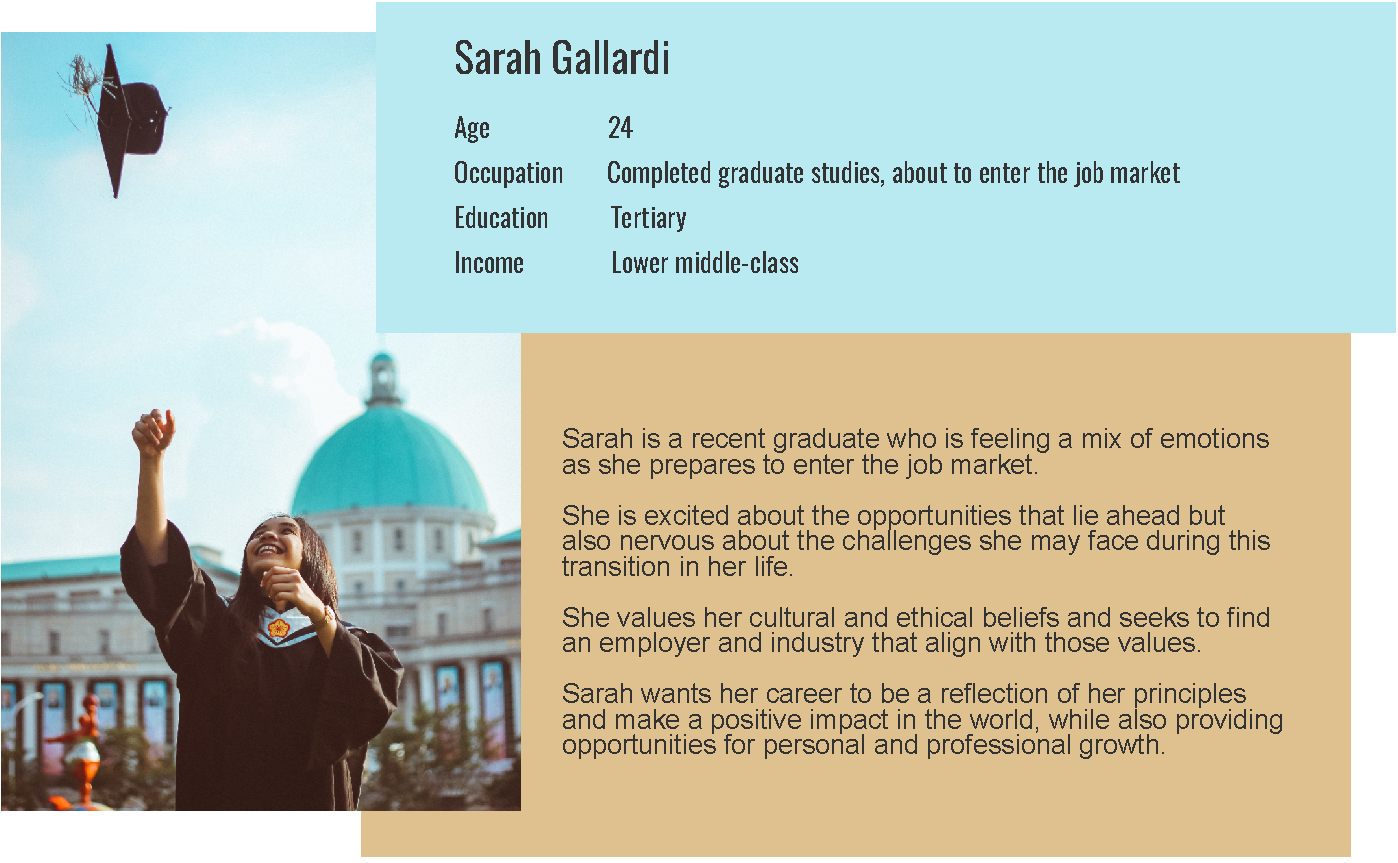
\includegraphics[width=\linewidth]{persona.pdf}
\end{figure}

\noindent\textbf{Goals and Needs:}

\begin{itemize}
    \item \textbf{Cultural and Ethical Alignment:} Sarah places a high value on cultural and ethical alignment with potential employers and certain industries. She seeks organizations that promote diversity, inclusion, and equality. She wants to work in an environment that respects and values different perspectives and cultures.
    \item \textbf{Sustainable Practices:} Sarah is passionate about sustainability and environmental responsibility. She is keen on working in industries that prioritize sustainable practices, such as renewable energy, green technologies, or eco-friendly initiatives. She wants to contribute to a better future through her career choices.
    \item \textbf{Social Impact:} Sarah wants her work to have a positive impact on society. She seeks opportunities in industries such as nonprofit organizations, social enterprises, or companies with a strong corporate social responsibility focus. She wants to make a difference and improve the lives of others through her career.
    \item \textbf{Ethical Business Conduct:} Sarah believes in conducting business ethically and responsibly. She values organizations that prioritize transparency, integrity, and ethical decision-making. She wants to work for employers who uphold high ethical standards and prioritize the well-being of employees and stakeholders.
    \item \textbf{Cultural Diversity and Inclusion:} Sarah values workplaces that foster cultural diversity and inclusion. She seeks employers who celebrate and embrace individuals from different backgrounds, perspectives, and experiences. She wants to work in an environment that promotes equality and offers equal opportunities for career growth.
    \item \textbf{Work-Life Balance:} Sarah recognizes the importance of work-life balance in maintaining her well-being and overall satisfaction. She prefers employers and industries that prioritize a healthy work-life balance, offer flexible working arrangements, and support employee well-being initiatives.
    \item \textbf{Learning and Development:} Sarah seeks employers and industries that prioritize continuous learning and development. She values organizations that provide opportunities for professional growth, training programs, mentorship, and support for employees' career advancement.
\end{itemize}

\noindent\textbf{Summary:}
Overall, Sarah wants to find an employer and industry that not only align with her cultural and ethical values but also provide
opportunities for personal and professional growth. She aspires to contribute to a sustainable, socially responsible, and inclusive
work environment where she can make a positive impact and thrive in her career.
Considering Maslow's hierarchy of needs, Sarah is currently in the process of fulfilling her basic needs by seeking an employment
that will secure food, shelter, etc. However, she also has highers aspirations: she strives to fulfill her psychological needs, such as
belongingness and esteem. The right job with the right employer will provide her with a sense of belonging and self-esteem. She wants to
feel valued and appreciated for her contributions, while being able to her career. Finally, aligning her cultural and ethical values with
her career choices will allow her to partly fulfill her self-actualization needs.


%%% Drivers
\newpage
\section{Drivers}
\label{sec:drivers}

\subsection{Human Drivers}

\subsection{Customer Drivers}

\subsubsection{Value Proposition Canvas}

\subsubsection{Persona}

\subsubsection{Customer Jobs}

\subsubsection{Pains}

\subsubsection{Gains}


%%% Enablers
\newpage
\section{Enablers}
\label{sec:enablers}

\subsection{Uniqueness \& Operational Excellence}

\subsection{Gain Creators}

\subsection{Pain Relievers}

\subsection{Customer Centricity: Addressing Customer Needs}

\subsection{Need For Collaboration \& Co-creation}


%%% Business Model
\newpage
\section{Business Model}
\label{sec:business_model}

\subsection{Business Model Canvas}

\subsection{Customer Segments}

\subsection{Value Proposition}

\subsection{Channels}

\subsection{Customer Relationships}

\subsection{Key Activities}

\subsection{Key Resources}

\subsection{Key Partnerships}

\subsection{Cost Structure}

\subsection{Revenue Streams}




%%% Contribution from Innovation
\newpage
\section{Contribution}
\label{sec:contribution}

\subsection{Business Idea}

\subsection{Assessment of the Innovation}

\subsection{Digital Ecosystem Fit}


%%% Evaluation
\newpage
\section{Evaluation}
\label{sec:evaluation}

%%% System Fit
\newpage
\section{System Fit}
\label{sec:system_fit}

\subsection{Fit of Uniqueness}

\subsection{Fit of Management}

\subsection{Fit of Structure}

\subsection{Fit of Partnering}

\subsection{Fit of Customer Understanding}


%%% Conclusions
\newpage
\section{Conclusion}
\label{sec:conclusion}

%%% References
\newpage
\bibliography{references}

%%% List of Figures
\newpage
\listoffigures

%%% List of Tables
\newpage
\listoftables

%%% Appendix
\newpage
\appendix
\section*{Appendix}
\label{sec:appendix}

\end{document}